 \documentclass[11pt]{article}

% Packages
\usepackage{sectsty}
\usepackage{graphicx}
\usepackage{listings}
\usepackage{amsmath}
\usepackage{courier}
\usepackage{float}
\usepackage{parskip}
\usepackage{wrapfig}
% Section Font Size
\lstset{basicstyle=\footnotesize\ttfamily,breaklines=true}

% Graphics Path
\graphicspath{ {./images/} }

% Margins
\topmargin=-0.45in
\evensidemargin=0in
\oddsidemargin=0in
\textwidth=6.5in
\textheight=9.0in
\headsep=0.25in

\title{Practical Work 1: TCP File Transfer}
\author{ BI12-076 Mai Hai Dang }
\date{\today}

\begin{document}
\maketitle

\section{Objective}
Create a file transfer application using TCP/IP protocol in CLI using one server, one
client and one socket connection. Then write a report to describe the implementation
using figures and code snippets.

\section{Socket}

The nodes are divided into two categories: server and client. Both have the same
step of creating a socket to communicate with each other, set up with the address
structure and bind to the address. The server will listen to the incoming connection
from the client and accept the connection. The client will connect to the server and
send the file to the server. The server will receive the file and save it to the
specified location.

\begin{figure}[H]
  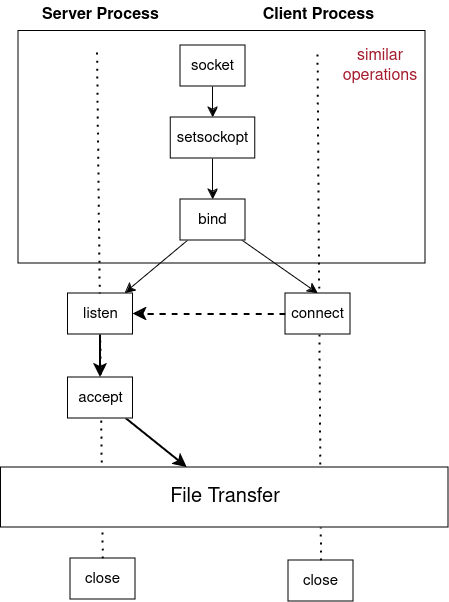
\includegraphics[scale=0.4]{socket.png}
  \centering
  \caption{Socket}
\end{figure}

\section{Protocol}
By definition, TCP is a connection-oriented protocol that provides reliable, ordered, 
and error-checked delivery of a stream of bytes between applications running on hosts 
communicating over an IP network. It is a transport layer protocol in the OSI layer 
and is used to create a connection between a client and a server.

We create a similar handshake protocol to establish a connection between the server and 
client. The server will listen to the incoming connection from the client. The client will 
send a connection request to the server. The server will accept the connection and send a 
acknowledgement to the client. Every step of sending and receiving data is also acknowledged.

\begin{figure}[H]
  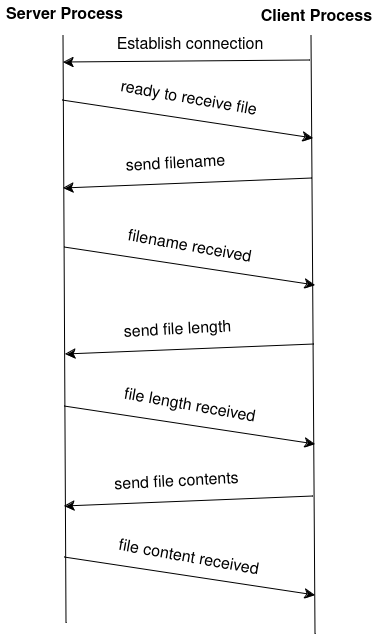
\includegraphics[scale=0.5]{file-transfer.png}
  \centering
  \caption{Protocol}
\end{figure}

% \begin{lstlisting}
% LogComponentEnable("UdpEchoClientApplication", LOG_LEVEL_FUNCTION);
% LogComponentEnable("UdpEchoServerApplication", LOG_LEVEL_FUNCTION);
% \end{lstlisting}

% \begin{figure}[H]
%   \includegraphics[scale=0.25]{template.png}
%   \centering
%   \caption{Logging output with DataRate = 5Mbps and Delay = 1ms}
% \end{figure}

\end{document}
